\chapter{Timers}
Before explaining how timers work, let's try to understand why we would need them.\\

Up until now, when we have wanted events to occur some human-scale time (hundreds or thousands of milliseconds) apart, we have been using long but finite loops to create delays. 
The delay loops have been incrementing or decrementing a number in a CPU register many thousands of times; a task which takes an appreciable amount of time to complete. This can be considered a waste of CPU resources. Instead of getting the CPU to do some useful work (controlling a system or monitoring some external signals) it is simply modifying an internal register for a long time. 
Clearly if we could create our delays or periodic events by some other method it would free up our CPU to be able to do other useful things. 
A timer satisfies this need.\\


A timer is a peripheral inside the microcontroller. 
We have about 8 different timers on our micro, each with a number. 
They range from advanced timers to basic timers. 
The advanced timers have all of the functionality of the basic timers plus a whole lot more functionality for doing fancy things. 
We will only consider the basic timers in this course as they have the simplest block diagrams and are easiest to understand. 

Essentially a timer is a configurable hardware counter. It has a register called the \textbf{CNT} (count) register which \emph{automatically} (without CPU intervention) counts up to a certain value and then starts counting up again from 0. 
The value which it counts up to is controlled by another register, the \textbf{ARR} (auto reload register). 
When the value in the CNT register becomes equal to the value in the ARR, the timer triggers an event called an Update Event or Overflow Event.
This event can in turn trigger an interrupt which in turn can get the CPU to jump to executing some specific block of code. 

\section{Basic Block Diagram}
The best way to understand how a timer is implemented and works is to consider the block diagram. The block diagram for the basic timer, timer 6 is shown in \autoref{fig:timer_basic_diagram}.

\begin{figure}
\centering
\includegraphics[page=508, clip=true, trim=195 270 135 430, width=\textwidth]{./stm32f0xx_reference_manual}
% left, bottom, right, top
\caption{Block Diagram of Basic Timer 6. Source: Figure 192, Reference Manual}
\label{fig:timer_basic_diagram}
\end{figure}

This block diagram shows additional information which the brief discussion above did not contain, namely the source of the clock frequency and an additional block called the \textbf{PSC} (prescaler). Following is a brief discussion on these aspects.

\subsection{Clock from RCC}
We know that the timer is centred around a counter which needs to have a well defined frequency. There is a clock line which enters the timer peripheral from the RCC. By default this line is running at 8 MHz. This the TIMxCLK line in the diagram. 

Should it be necessary you could modify the timer clock frequency independently of the frequency of other peripherals or the CPU. 
This is functionality provided by the RCC. 

\subsection{Control}
The control block configures how the timer will work. This includes such aspects as:
\begin{itemize}
\item whether the TIMxCLK line is allowed to pass through the control block to the next blocks (counter enabled) or if the TIMxCLK line is prevented from going further (counter disabled).
\item whether the timer will generate an interrupt when an overflow event happens
\item whether or not registers are shadowed
\item and many more
\end{itemize}

There are registers which we modify in order to configure the control block. These will be discussed shortly. 

\subsection{Prescaler}
A prescaler is essentially a frequency divider. A clock line with a certain frequency enters the prescaler. The clock line exiting the prescaler has a frequency equal to the input frequency divided by some factor. 

Prescalers are very common and useful in digital systems so it is worth discussing them a bit. A prescaler is essentially characterised by the range of values which it is able to divide by. Simple prescalers (such as those contained in the RCC block) are only able to divide by a select few powers of 2 (example, 1, 2, 8, 32, 128). Other prescalers (such as the one in our timer block) are able to divide by any integer in a certain range. Our timer PSC block has 16 bits worth of configurable prescaling so it can divide by anything from 0 to $2^{16} - 1$ = 65535. This prescaler which can divide by arbitrary integers is obviously more powerful than one with a very small number of values, but require more transistors to manufacture (ie: costs more). 

There is a slight additional complication: the value which the prescaler actually divides by is equal to the value which it has been programmed with \emph{plus 1}. The reason for this is to avoid the division-by-zero case for when the prescaler is programmed with 0. In other words, if you place the value 0 into the prescaler it will actually divide by 1 (leave the signal unchanged). 

Values are placed into the prescaler by writing to the TIMx\_PSC register.

\section{Timer Interrupts}
We know that the timer CNT register will count up to the value in the ARR, starting from 0.
When CNT equals ARR, overflow happens and the CNT is reset to 0. 
Hence, there are ARR + 1 counts which happen.
Additionally, an Update Event (UE) will generally be generated. 
This update event can optionally cause an Update Interrupt (UI).\\

An interrupt is similar to an \emph{exception} (discussed in \autoref{sec:exceptions}). Typically an interrupt is generated by a peripheral while an exception is generated by the system with something bad happens. When an interrupt occurs, the usual exception handling procedure takes place: the CPU stacks its system state and fetches the vector for that exception. It then executes the code specified by the exception. Table 33 of the Reference Manual shows the addresses of the vectors of each peripheral which can generate interrupts. 

When a timer triggers an interrupt, the CPU does not always respond to it. This is because there is a block between the peripheral and the CPU: the NVIC. This will be discussed more in the next section.

Assuming the timer has been configured to generate an interrupt and the NVIC has been configured to allow the interrupt, the CPU will jump to executing the ISR when overflow happens.

\subsection{Acknowledging Interrupts} 
The timer peripheral will keep asserting its interrupt request until the interrupt has been acknowledged. 
In other words, until the CPU has said to the timer: "I have dealt with your interrupt request." 
The CPU does not automatically inform the timer when its interrupt is being handled.
Instead, this must be done by your code.
To acknowledge the interrupt, your interrupt handler code must write a 0 to the UIF bit in the TIMx\_SR.
Only once this happens will the peripheral clear its interrupt request.
If you do not acknowledge the interrupt, the ISR will be run again immediately after it finishes \emph{ad infinitum}. 

It is advised to acknowledge the interrupt as the first action of the ISR.

\section{Frequency/Period Calculation}
We know that the timer is clocked by an 8 MHz source by default. That source is then divided by PSC + 1. With that in mind, the time interval each tick of the CNT register is as follows.
\begin{equation}
    t_{CNT} = \frac{1}{f} = \frac{1}{\frac{\SI{8}{MHz}}{\text{PSC} + 1}} = \frac{\text{PSC} + 1}{\SI{8}{\mega\hertz}}
\end{equation}

Of course you will need to adjust that equation should it be specified that the timer is clocked by a different frequency.

We know that each tick of the CNT register happens after time $t_{CNT}$ as calculated above. We know that the timer will count from 0 to the value in the ARR before overflow happens. 
Hence, we know that the time between overflows is equal to:
\begin{equation}
  t_{OVERFLOW} = t_{CNT} \times (\text{ARR} + 1) = \frac{(\text{PSC} + 1) \times (\text{ARR} + 1)}{\SI{8}{\mega\hertz}}
\end{equation}

Naturally, the frequency of overflow events is the inverse of the above.
